\section{Cross validation}
When training machine learning models it is important to split your data into three categories, training, validation and test. The training set is the data the model is trained on, and models will tend to overfit this data. Because of this, we use a validation set to validate that the model generalizes to unknown data, that is, we do not train on the validation data, we only evaluate performance on it. The test set is only used at the very end when the final model evaluation is performed. If we have loads of data, we can simply split our data into these three categories and keep them static. But if we only have a small dataset we can use the cross validation technique. Here our data is split into a training set and a test set. The test set is as always only used at the very end. However, the training set is then further divided into 'splits'. A series of 'folds' are then performed. At each fold, one split is kept as a validation set and the rest is used as training data. As we complete a fold we move to the next where a new split is used as validation set and the rest is used as training data. Using this approach, each split will eventually be held out and used as validation data. At the end, the model performance is evaluated on the test set. Using this approach we utilize our data more efficiently and is to prefer when we have very little data to work with. However, as we still train on our validation data we do not get as accurate an indication of how good the model generalizes on unknown data. Also more care needs to be taken when using cross validation as we need to ensure each fold has the same proportion of observations with a certain property. When creating static data sets we only need to ensure this for the three data sets, but for cross validation we need to ensure this for each of the \textit{k} folds plus the test set. An illustration of cross validation can be seen in \autoref{crossVal}.
\begin{figure}
	\centering
	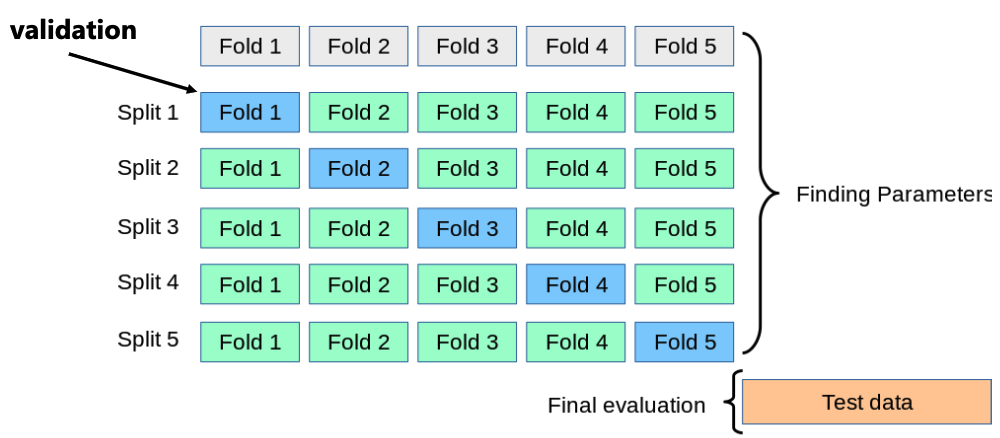
\includegraphics[width=0.83\linewidth]{Materials/crossValidation}
	\caption{Illustration of cross validation. Each of the blue splits are used at turn as validation sets, whereas the green splits are used training sets. Illustration taken from slides.}
	\label{crossVal}
\end{figure}